% Draft, 2026-11-25. Concept unlearning without the source data; all numbers from colab_results/gate5 and gate6.
% Overleaf: compiler pdfLaTeX. Figures in figures/: trajectory_s0.png, relearn_s0.png.
\documentclass[conference]{IEEEtran}
\usepackage[utf8]{inputenc}
\usepackage[T1]{fontenc}
\usepackage{amsmath,amssymb}
\usepackage{graphicx}
\usepackage{booktabs}
\usepackage{xcolor}
\usepackage{url}
\usepackage[hidelinks]{hyperref}

\newcommand{\tbd}[1]{\textcolor{red}{[TBD: #1]}}
\newcommand{\figorbox}[2]{\IfFileExists{#1}{\includegraphics[width=\columnwidth]{#1}}{\fbox{\parbox[c][#2][c]{0.95\columnwidth}{\centering\small\textcolor{red}{missing #1}}}}}
\newcommand{\tref}{\theta_{\text{ref}}}
\newcommand{\tb}{\theta_{\text{b}}}
\newcommand{\ten}{\theta_{\text{en}}}

\begin{document}

\title{Unlearning a Concept Without Its Training Data:\\Removing English from a Character-Level Portuguese Transformer}

\author{\IEEEauthorblockN{Laura Pontiroli Machado}
\IEEEauthorblockA{Computer Science, Insper\\laurapm@al.insper.edu.br}}

\maketitle

\section{Introduction}
Removing knowledge from a model is needed for privacy, copyright and safety. Exact unlearning retrains without the data~\cite{bourtoule2021}, which requires knowing which data taught the model and is rarely affordable. Many requests concern a concept (a language, a dangerous topic, a style) whose sources in a web-scale corpus cannot be listed; one can only collect new examples and unlearn on them. Approximate methods update the weights directly: gradient ascent (GA) on the forget set~\cite{jang2023}, ascent plus descent on retained data (NegGrad+)~\cite{kurmanji2023}, or preference-style losses~\cite{zhang2024npo}. They are evaluated against retrained models or benchmark proxies~\cite{maini2024tofu}, and ``unlearned'' knowledge often returns after brief fine-tuning~\cite{lynch2024eight}.

\textbf{Question.} Can a concept be unlearned from examples, without the data that taught it? I use a language as the concept because it is broad and easy to sample and measure. Since English is added \emph{after} Portuguese, the Portuguese-only ancestor $\tref$ is an exact target that needs no retraining. Forgetting is measured on held-out English, so it is forgetting of the concept, not of passages. \textbf{H1}: GA damages Portuguese before English reaches $\tref$'s level. \textbf{H2}: NegGrad+ matches $\tref$ on English while keeping Portuguese, but English is relearned faster than from $\tref$. \textbf{H3}: fine-tuning on Portuguese alone forgets less English than NegGrad+. \textbf{H4} (added after H1--H3): unseen English unlearns as well as training-pool English.

\section{Method}
\textbf{Data and models.} Portuguese (PT) and English (EN) Wikipedia~\cite{wikipedia}, split by title hash and lowercased into 62 symbols: 80M training and 2M validation/test characters per language, plus 5M fresh EN characters. The model is a 6-layer, $d{=}256$ transformer~\cite{vaswani2017,nanogpt} (4.9M parameters, context 512). $\tref$ is trained on PT for 6000 steps; $\tb$ continues for 1800 steps on 32 PT + 32 EN sequences per step.

\textbf{Unlearning.} From $\tb$, with $L_x$ the cross-entropy on batch $x$: M1 (control) minimizes $L_{PT}$, M2 (GA) $-L_{EN}$, M3 (NegGrad+) $-L_{EN}+\lambda L_{PT}$, with 32 EN + 32 PT sequences per step (AdamW, at most 1000 steps). A run stops when $L_{EN}$ exceeds $\ln 62+1$ nats (worse than uniform). Grid: lr $\in\{2,5\}\cdot10^{-5}$ and $\lambda\in\{1,2\}$ for M3; lr $5\cdot10^{-5}$ for M1, M2. EN comes from $\tb$'s training pool; the \emph{proxy} run (H4) repeats the selected M3 with fresh EN no model has seen. The unlearning code never loads $\tref$ (checked by a test). The \emph{practitioner} point is the last checkpoint (every 5 steps) before PT validation bpc rises 2\% above $\tb$'s; the \emph{oracle} point, an upper bound, is the first whose EN validation bpc reaches $\tref$'s.

\textbf{Evaluation.} Bits per character (bpc) and per-character $\mathrm{KL}(p_{\text{ref}}\|p_\theta)$ on 500 test chunks per language; from 200 prompts per language, \emph{EN leakage} (EN-only over EN-only + PT-only generated words) and real-word rate. For relearning, models are fine-tuned 300 steps on PT only or on PT + 1M fresh EN characters; the \emph{dormancy gap} is $\tref$'s EN bpc minus the unlearned model's (positive = suppressed, not removed). Choices use validation data; each model is tested once. CIs are 95\% bootstrap over chunks (paired between models).

\section{Results}
$\tref$ reaches 1.620 bpc on PT test and 2.480 on EN. $\tb$ lowers EN to 1.808 with PT at 1.637, but its PT text holds 18$\times$ more English. The EN gap to close is 0.672 bpc.

\begin{figure}[t]
\centering
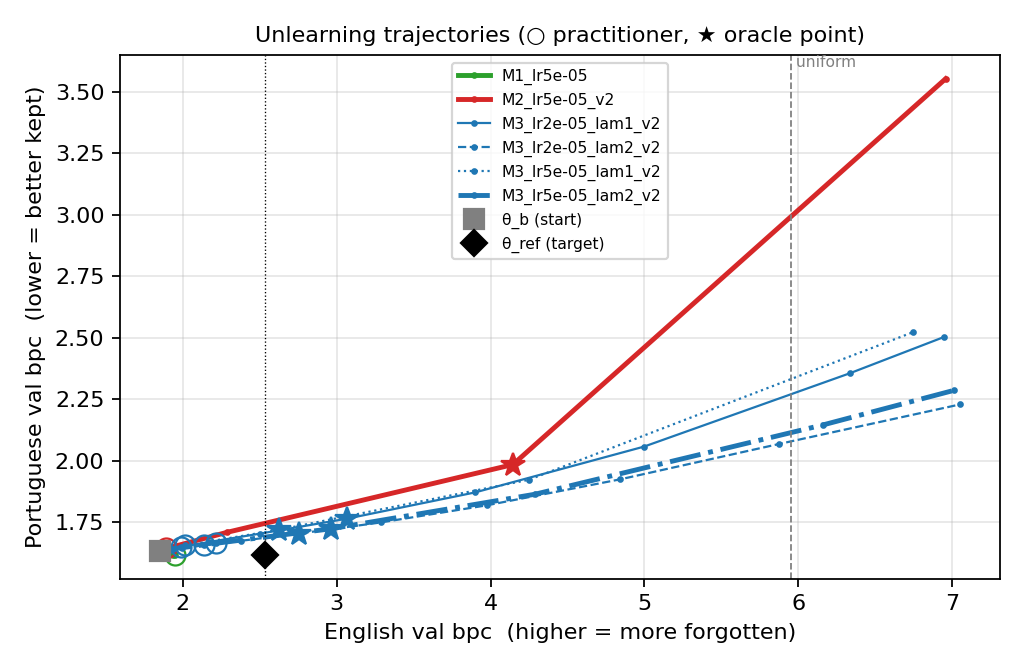
\includegraphics[width=0.8\columnwidth]{figures/trajectory_s0.png}
\caption{Unlearning trajectories on validation data, from $\tb$ (square) toward $\tref$ (diamond). Circles: practitioner points; stars: oracle points.}
\label{fig:traj}
\end{figure}

\begin{table}[t]
\centering
\caption{Test results (seed 0; bpc CIs $\pm$0.02--0.045). KL to $\tref$ in bits/char; Leak: EN leakage from PT/EN prompts; Real: real-word rate. Practitioner point unless (or.) = oracle.}
\label{tab:main}
\setlength{\tabcolsep}{2.5pt}
\footnotesize
\begin{tabular}{lccccccc}
\toprule
Model & PT & EN & KL$_{PT}$ & KL$_{EN}$ & Leak$_{PT}$ & Leak$_{EN}$ & Real \\
\midrule
$\tref$ & 1.620 & 2.480 & 0 & 0 & 0.002 & 0.064 & 0.94\\
$\tb$ & 1.637 & 1.808 & 0.054 & 0.820 & 0.036 & 0.975 & 0.94\\
\midrule
M1 control & 1.618 & 1.901 & 0.037 & 0.441 & 0.005 & 0.304 & 0.93\\
M2 GA & 1.645 & 1.850 & 0.061 & 0.795 & 0.024 & 0.941 & 0.92\\
M2 (or.) & 1.983 & 4.137 & 0.398 & 2.600 & 0.041 & 0.825 & 0.69\\
M3 NegGrad+ & 1.669 & 2.168 & 0.074 & 0.525 & 0.002 & 0.030 & 0.93\\
M3 (or.) & 1.729 & 2.913 & 0.127 & 0.887 & 0.001 & 0.008 & 0.90\\
\midrule
M3 proxy & 1.651 & 1.952 & 0.061 & 0.665 & 0.003 & 0.181 & 0.93\\
M3 proxy (or.) & 1.773 & 3.330 & 0.165 & 1.296 & 0.000 & 0.011 & 0.91\\
\bottomrule
\end{tabular}
\end{table}

\begin{figure}[t]
\centering
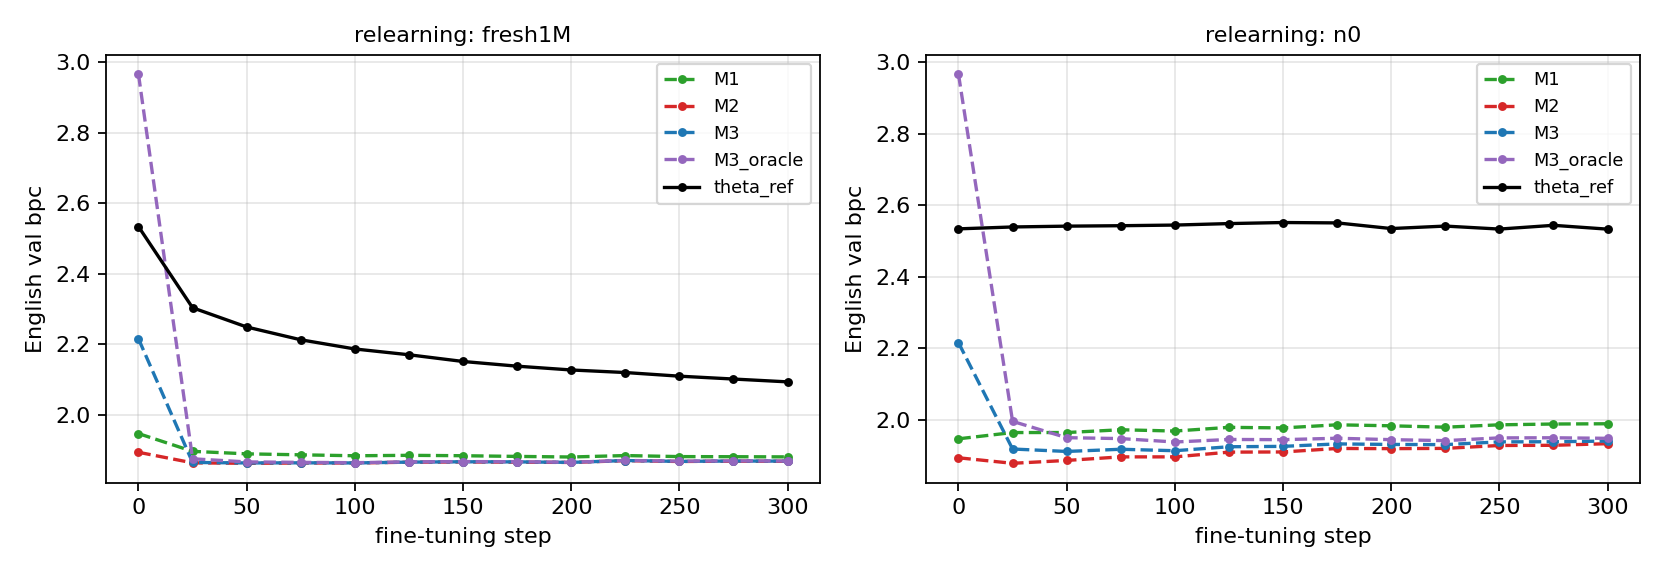
\includegraphics[width=\columnwidth]{figures/relearn_s0.png}
\caption{Relearning: EN validation bpc during fine-tuning on PT + 1M fresh EN (left) and on PT only (right).}
\label{fig:relearn}
\end{figure}

\textbf{H1 (supported).} Every ascent-based run hit the guard within 66 steps; GA at step 21, with a usable window of about 5 steps. When its EN bpc passes $\tref$'s, it overshoots to 4.14 and PT has risen by 0.36 bpc (69\% real words).

\textbf{H2 (partly supported).} NegGrad+ ($5\cdot10^{-5}$, $\lambda{=}2$) closes 54\% of the EN gap at its practitioner point (others: 20--42\%) for +0.032 PT bpc (paired CI [0.029, 0.035]). At the oracle point PT costs +0.11 over $\tref$, and its EN KL (0.89) is \emph{higher} than $\tb$'s (0.82): matching bpc is not matching the distribution.

\textbf{H3 (bpc yes, KL no).} The control raises EN bpc by only 0.09 (NegGrad+: 0.36), yet it is closest to $\tref$ in both languages (KL 0.037 PT, 0.44 EN); ascent moves PT \emph{away} from $\tref$. Leakage overstates forgetting: NegGrad+ leaks less English than $\tref$ (0.030 vs.\ 0.064) while closing half the bpc gap.

\textbf{Relearning} (Fig.~\ref{fig:relearn}). With 1M EN characters, every unlearned model, including the oracle model starting at 2.97, is back at 1.86--1.90 EN bpc within 25 steps ($\tb$: 1.85); $\tref$ only reaches 2.30, then 2.09 at step 300 (gap +0.44, +0.23). With PT only, $\tref$ stays at 2.53, but NegGrad+ regains English without seeing any: 2.22$\to$1.92 and 2.97$\to$2.00 within 25 steps (gap +0.59 at 300).

\textbf{H4 (supported).} With unseen English, NegGrad+ follows the same trade-off curve: at $\tref$'s EN level, PT is 1.692 vs.\ 1.690; it collapses at step 30 (vs.\ 33). Its relearning matches too: with PT only it returns to 1.90 (practitioner) and 2.04 (oracle) within 25 steps; the gap is +0.60 at 300.

\section{Conclusion}
\textbf{So what.} Unseen English worked exactly as well as the training pool, so missing source data was not the obstacle. But no method removed English. By leakage NegGrad+ beats $\tref$, by bpc it is halfway, and by KL it is further from $\tref$ than a Portuguese-only fine-tune; a few Portuguese steps bring its English back. Unlearning moved the model to a new state that suppresses the concept, not to one that never learned it. Without source data or a retrained model, evaluations should include distributional distance and relearning, not only forget loss or generation. \textbf{Limitations.} One seed, one small model, a reduced grid; PT Wikipedia contains some English; H4 was added after the main results. \textbf{What I learned.} The metric decides whether unlearning looks successful, so an exact reference is worth building; and ascent needs dense monitoring, since the useful window was 5--20 of 1000 planned steps.

\section{Use of AI}
I found related work by asking Claude (Anthropic) for key papers and talks on machine unlearning, studying them, and briefly discussing the topic with researchers in the area. An AI coding assistant (Claude Code) did the routine work: it wrote and tested the code (data, training, unlearning, evaluation, Colab notebooks) and drafted and formatted this report. I set the question, hypotheses and scope, approved each stage before the next ran, approved the design changes it proposed (logged as deviations), ran all experiments and checked the results and text.

\bibliographystyle{IEEEtran}
\bibliography{refs}
\end{document}
